\documentclass[tikz, border=7pt]{standalone}
\usepackage{tikz}

\begin{document}
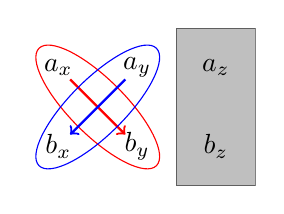
\begin{tikzpicture}[scale=1]

  \node at (0,1) {$a_x$};
  \node at (0,0) {$b_x$};

  \draw [fill=gray, opacity =0.5] (1.5, -0.5) rectangle (2.5,1.5) ;

  \node at (1,1) {$a_y$};
  \node at (1,0.0) {$b_y$};

  \node at (2,1) {$a_z$};
  \node at (2,0) {$b_z$};

  \draw[rotate around={45:(0.5,0.5)},red] (0.5,0.5) ellipse (10pt and 30pt);

  \draw[->, red, thick] (0.15,0.85) -- (0.85,0.15);

  \draw[rotate around={-45:(0.5,0.5)},blue] (0.5,0.5) ellipse (10pt and 30pt);

  \draw[->, blue,thick] (0.85,0.85) -- (0.15,0.15);

\end{tikzpicture}
\end{document}
